\documentclass{article}
\usepackage[utf8]{inputenc}
\usepackage{tikz}
\usepackage{longtable}
\usepackage{amsmath}

%% pdflatex exempleSortie.tex && rm *.aux *.log

\title{Brain Map of Norn}
\author{Creatures Genome Analyzer}
\date{\today}

\begin{document}
\maketitle

\section*{Brain Map}

\begin{center}
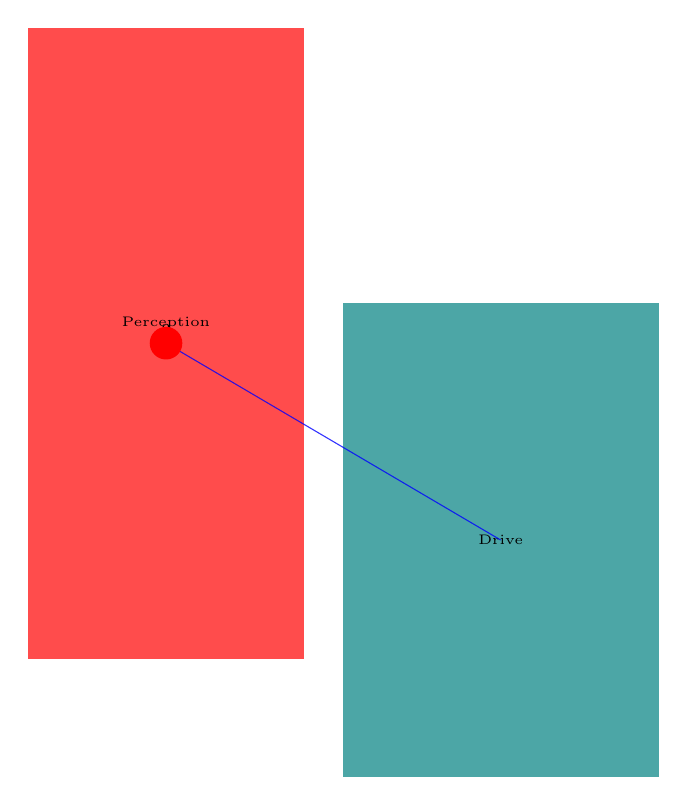
\begin{tikzpicture}[scale=0.5]
\filldraw[red!70] (4,13) rectangle (11,29);
\node at (7.5,21.5) {\tiny Perception};
\filldraw[teal!70] (12,10) rectangle (20,22);
\node at (16,16) {\tiny Drive};
\draw[blue, opacity=0.8] (7.5,21) -- (16,16);
\filldraw[black] (7.5,21) circle (0.2);
\node at (7.5,21) [above, font=\tiny] {2};
\filldraw[red] (7.5,21) circle (0.4);
\end{tikzpicture}
\end{center}

\newpage

\section*{Dendrites Legend}

\begin{longtable}{|p{3cm}|p{3cm}|p{3cm}|p{3cm}|}
\hline
{\bf Source} & {\bf Target} & {\bf Strength} & {\bf Type} \\ \hline
Perception[0] & Drive[0] & 200 & D0 \\ \hline
\end{longtable}

\section*{Instincts Legend}

\begin{longtable}{|p{3cm}|p{3cm}|p{3cm}|p{3cm}|}
\hline
{\bf Action} & {\bf Reward/Punish} & {\bf Amount} & {\bf Conditions} \\ \hline
Come & Reward & 5 & Drive[2], Verb[1], General Sense[0] \\ \hline
\end{longtable}

\section*{Chemical Reactions}

\begin{longtable}{|p{4cm}|p{4cm}|p{2cm}|}
\hline
{\bf Reactants} & {\bf Products} & {\bf Rate} \\ \hline
1 Pain + 1 Hunger & 1 Reward + 1 Energy & 5 \\ \hline
\end{longtable}

\section*{Chemical Half-Lives}

\begin{longtable}{|p{4cm}|p{4cm}|}
\hline
{\bf Chemical} & {\bf Half-Life} \\ \hline
Pain & 10 \\ \hline
Hunger & 20 \\ \hline
\end{longtable}

\end{document}
